\chapter{Evaluation vorhandener Lösungsalternativen}\label{chap:eval}
Im folgenden Kapitel werden drei Lösungsalternativen aus dem Google Play-Store zur Aufmaßerfassung vorgestellt und evaluiert.
Hierzu werden die Bewertungskriterien zunächst vorgestellt, und anschließend iterativ auf die ausgewählten Apps angewandt.
Dieses Kapitel schließt die \emph{Observation} Phase ab, welche in \autoref{chap:problem} begonnen wurde. 

\section{Bewertungskriterien}
Zur Evaluation der Lösungsalternativen wird die erweiterte Version der Nielsen-Heuristiken \citep{Nielsen94}, sowie eine zusätzliche Menge selbst aufgestellter Kriterien benutzt \todo{anders schreiben}.
Da sich die erweiterten Nielsen-Heuristiken aus 18 verschiedenen Kriterien zusammensetzen, von denen nicht jede bezüglich des Einsatzbereiches im Gerüstbau gleich relevant ist, werden die Kriterien nach Absprache mit der Geschäftsleitung in zwei Klassen eingeteilt (R = als relevant beurteil, I = als nicht relevant beurteilt).
Für die Evaluation der Apps werden anschließend nur Kriterien benutzt, die in diesem Kontext als relevant klassifiziert wurden.
\todo{Gewichtung überarbeiten}

\subsection{Die erweiterten Nielsen-Heuristiken}\label{subsec:nielsen}
\citeauthor{Nielsen94} führt in seinem Buch ``Usability inspection methods'' zehn Heuristiken auf, die auf einer Grundlage von allgemein anerkannten Prinzipien beruhen, und sich zur Evaluation von Usability-Problemen besonders gut eignen \citep[Seiten 25--62]{Nielsen94}: 

\begin{enumerate}
    \di{Sichtbarkeit des Systemzustandes (R)}{N1}{Angemessene Rückmeldung in einem vernünftigen zeitlichen Rahmen}
    \di{Übereinstimmung zwischen System und realer Welt (R)}{N2}{Sprache des Benutzers, natürliche und logische Reihenfolge}
    \di{Benutzerkontrolle und -freiheit (R)}{N3}{Undo und Redo}
    \di{Konsistenz und Standards (R)}{N4}{Konsistente Nutzung und Beachtung der Plattform-Konventionen}
    \di{Fehlervorbeugung (R)}{N5}{Vermeide Situationen in denen Fehler entstehen können}
    \di{Wiedererkennung statt Erinnern (R)}{N6}{Objekte, Optionen und Aktionen sollen sichtbar sein}
    \di{Flexibilität und Effizienz der Benutzung (R)}{N7}{Häufige Aktionen anpassbar, Experten schnellere Bedienung erlauben}
    \di{Ästethisches und minimalistisches Design (I)}{N8}{Keine irrelevanten Informationen}
    \di{Erkennbarkeit, Diagnose und Erholung von Fehlern (R)}{N9}{Verständliche Fehlermeldungen}
    \di{Hilfe und Dokumentation (R)}{N10}{Leicht zu finden, abgestimmt auf Aufgabe, konkrete Schritte zur Lösung}
\end{enumerate} 

\noindent
Zur Bewertung von Software auf mobilen Endgeräten reichen diese zehn Bewertungskriterien jedoch nicht vollständig aus, sodass acht weitere Heuristiken, die speziell für mobile Geräte ausgelegt sind, hinzugezogen werden \citep{Bertini06}.
\citeauthor{MachadoNeto13} schlagen hierzu in ihrem Artikel ``Heuristics for the assessment of interfaces of mobile devices'' die folgenden weiteren Kriterien vor:

\begin{enumerate}
    \setcounter{enumi}{10}
    \di{Adäquater Umgang mit Unterbrechnungen (R)}{N11}{Kein Verlust von Informationen bei Unterbrechung der Aktivität}
    \di{Fokussieren der Informationen (R)}{N12}{Hervorheben der wichtigen Informationen, um schnelles Scannen zu erlauben}
    \di{``Joy of Use'' (R)}{N13}{Positives Nutzungserlebnis bei Bedienung/Verwendung}
    \di{``Don't lie to the user'' (I)}{N14}{Keine falschen oder ungültigen Zahlen, Fakten bzw. Nachrichten}
    \di{Unterstützung verschiedener Bildschirmausrichtungen (R)}{N15}{Keine Verwirrung bei verschiedenen Ausrichtungen des Bildschirms}
    \di{Ergonomische Gestaltung der physischen Interatkion (R)}{N16}{Kein unabsichtliches Auslösen von Funktionen}
    \di{Einfache Eingabe, Bildschirmlesbarkeit und Übersichtlichkeit (R)}{N17}{Einfache Navigations- und Eingabetechniken bei einhändiger Benutzung}
    \di{Stelle Privatheit sicher (I)}{N18}{Vermeide den Verlust/Diebstahl von privaten Daten z.b.\ durch Passwörter}
\end{enumerate}

\noindent
Bei der Klassifizierung der Kriterien wurden ``8. Ästethisches und minimalistisches Design'', ``14. Don't lie to the user'' und ``18. Stelle Privatheit sicher'' als nicht relevant gewichtet, da diese drei Punkte nach Absprache mit der Geschäftsleitung bei der Entwicklung einer eigenen Android-App für die Zielgruppe nicht wichtig seien.
\todo{warum wurden gerade diese als I markiert}

\subsection{Weitere Kriterien}
Zusätzlich zu den in \autoref{subsec:nielsen} vorgestellten Heuristiken werden noch zwei weitere Kriterien zur Evaluation hinzugezogen, die für die Einbindung in eine bereits bestehende Systemarchitektur wichtig sind: 

\begin{itemize}
    \di{Integration der App in eine vorhandene Systemarchitektur}{integration}{Die App sollte sich in eine bereits vorhandene Systemarchitektur leicht integrieren lassen}
    \di{Export des annotierten Bildes und der Metadaten zur Weiterverarbeitung durch einen nachgelagerten Dienst (z.B. \emph{API})}{export}{Die App sollte die eingetragenen Meta-Daten, wie zum Beispiel die Längen einer Linie, zur Weiterverarbeitung exportierbar machen}
    \todo{Hier noch mehr Kriterien auflisten}
\end{itemize}
\todo{Punkte beschreiben}

\section{Vorstellung und Evaluation ausgewählter Apps}\label{sec:evaluation}
Als Lösungsalternativen werden im folgenden drei Android-Applikationen vorgestellt, die unter dem Suchbegriff ``Aufmaße'' im Google Play-Store gelistet werden.
Bei der Auswahl der Lösungsalternativen wurden verschiedene Auswahlkriterien berücksichtigt.
So achtet, nach einer Studie aus dem Jahr 2014 von \citeauthor{Dogruel14}, in der 49 Smartphone-Nutzer bei ihrer Entscheidungsfindung zum Download von Apps aus dem Google-Play Store beobachten wurden, ein Großteil (74\%) der Testpersonen auf eine gute Bewertung der App.
33\% der Testpersonen stützen sich laut \citeauthor{Dogruel14} bei ihrer Entscheidungsfindung außerdem auch noch auf Rezensionen über die App.
Für 9\% der Testpersonen sei die Anzahl der Downloads bzw. die Popularität der Applikation ein weiteres Entscheidungskriterium \citep{Dogruel14}. \\

Um die Lösungsalternativen möglichst repräsentativ für das Angebot im Play-Store zu wählen, wurden Apps ausgewählt, die jeweils eine der oben genannten Auswahlkriterien besonders gut erfüllen.
Hierbei handelt es sich um die folgenden drei Apps:

\begin{itemize}
  \item \mm{} - Bosch GmbH (\textit{Popularität})
  \item \im{} - Dirk Farin (\textit{Bewertungen})
  \item \pm{} - Blue Big Pixel Inc. (\textit{Rezensionen})
\end{itemize}

\noindent
Die App \mm{} der Bosch GmbH stammt von einem internationalen Großkonzern mit mehr als 80 Standorten in Deutschland, und einem Jahresumsatz von 14,5 Mrd. Euro \citep{Bosch18}.
Mit zwischen 100 000 bis 500 000 Installationen gehört die App zu einer der Populärsten unter dem Suchbegriff ``Aufmaße'' im Google Play-Store.

\im{} von Dirk Farin wurde ausgewählt, da die App mit einer Gesamtbewertung von 3,9 von 5 Sternen bei 2 764 abgegebenen Bewertungen eine der beliebtesten Apps unter dem Suchbegriff ``Aufmaße'' ist.

Im Gegensatz dazu zeichnet sich die App \pm{} von Blue Bixel Inc. durch eine Vielzahl positiver Rezension aus, welche in der App-Beschreibung im Google Play-Store rezitiert werden.
So bewertet die Review-Seite ``App-Safari'' die App mit den Worten ``So incredibly convenient'' \citep{AppSafari18}, und auf der deutschen Seite ``appgefahren.de'' wird die App weiter gelobt:
``[...] für seinen Zweck eine richtige Empfehlung - die App macht genau das, was sie verspricht.'' \citep{Appgefahren18}.
Das Architektur- und Designmagazin ``Architectural Digest'' bewertet die App als ``very useful when shopping or meeting with contractors'' \citep{Architect18}. \\

Die Bewertungskriterien werden in den nachfolgenden Unterkapiteln jeweils in der Reihenfolge evaluiert, wie sie während des normalen Nutzungsablaufs der entsprechenden App aufgetreten sind.
\subsection{Measuring Master}

\subsubsection{Vorstellung}
\todo{Version, Downloaddatum, Playstore-Link}
Die App \mm{} von der Bosch GmbH ist im Play-Store unter der Rubrik ``Effizienz'' aufgelistet.
Selbst beschreibt der App-Hersteller seine Software wie folgt \citep{BoschMM}:

\begin{quote}
  ``Measuring Master ist eine multifunktionale App, die es ermöglicht, Aufmaße, Grundrisse und Temperaturmesswerte an einem Ort zu dokumentieren und zu verwalten.\\
  Die App ist besonders geeignet für Architekten, Maler, Bodenleger, Heizungsbauer und Elektriker, aber auch alle anderen Handwerker profitieren von der umfangreichen Funktionalität''
\end{quote}

\noindent
Nach dem Start der Applikation bietet sich die Möglichkeit ein neues Projekt anzulegen, oder bereits vorhandene Projekte zu bearbeiten.
Sobald das gewünschte Projekt ausgewählt wurde, bieten sich dem Benutzer über das Menü an der linken Seite diverse Funktionen (siehe \autoref{fig:bmenu}) an. \\

\begin{figure}[h]
  \centering
	\begin{subfigure}[t]{0.4\textwidth}
		\includegraphics[keepaspectratio, width=\textwidth]{bosch/menu}
		\caption{Navigationsmenü}
		\label{fig:bmenu}	
	\end{subfigure}
	\begin{subfigure}[t]{0.4\textwidth}
		\includegraphics[keepaspectratio, width=\textwidth]{bosch/bar}
		\caption{Aufmaße-Funktion}
		\label{fig:bbar}	
	\end{subfigure}
  \caption{\mm{} bei ausgeklapptem Navigationsmenü und in der Aufmaße-Funktion}
\end{figure}

Im Folgenden wird der Menüpunkt ``Aufmaße'' und die damit verbundene Funktionalität weiter vorgestellt und evaluiert.
So bietet sich dem Benutzer nach Auswahl der Aufmaße-Funktion die Möglichkeit, ausgewählte Bilder direkt mit Messwerten zu beschriften.
Hierzu können entweder Bilder direkt aus der Gallerie importiert, oder mit der Kamera aufgenommen werden.
Sobald der Benutzer den Foto-Import erfolgreich abgeschlossen hat, öffnet sich eine neue Ansicht, welche das ausgewählte Bild und weitere Bedienelement, in Form einer Statusleiste am unteren Rand, zeigt (siehe \autoref{fig:bbar}). \\

In dieser Benutzeroberfläche kann der Nutzer mit Hilfe von vier verschiedenen Formen (Linie, Viereck, Winkel, Freiform) Aufmaße ins Bild anzeichnen, und über einen Klick auf die gewünschte Form, Messwerte eintragen.
Außerdem bietet die App die Option, eine ausgewählte Reihe von Laserentfernungsmesser mit der App zu verbinden.
Dies ermöglicht eine Übertraung der gemessenen Distanzen über eine Bluetooth-Schnittstelle direkt an die App. \\

Um das annotierte Bild außerhalb der App weiter zu benutzen, bietet diese den Export als \emph{PDF} und \emph{JPEG} an.
Die exportierte \emph{PDF} enthält im Gegensatz zu der \emph{JPEG} zusätzlich zu dem annotierten Bild auch noch eine Tabelle mit allen eingetragenen Messwerten \autoref{fig:bexport}. 
Zudem lassen sich annotierte Bilder in der App speichern und zu einem späteren Zeitpunkt wieder bearbeiten.

\begin{figure}[h]
  \centering
  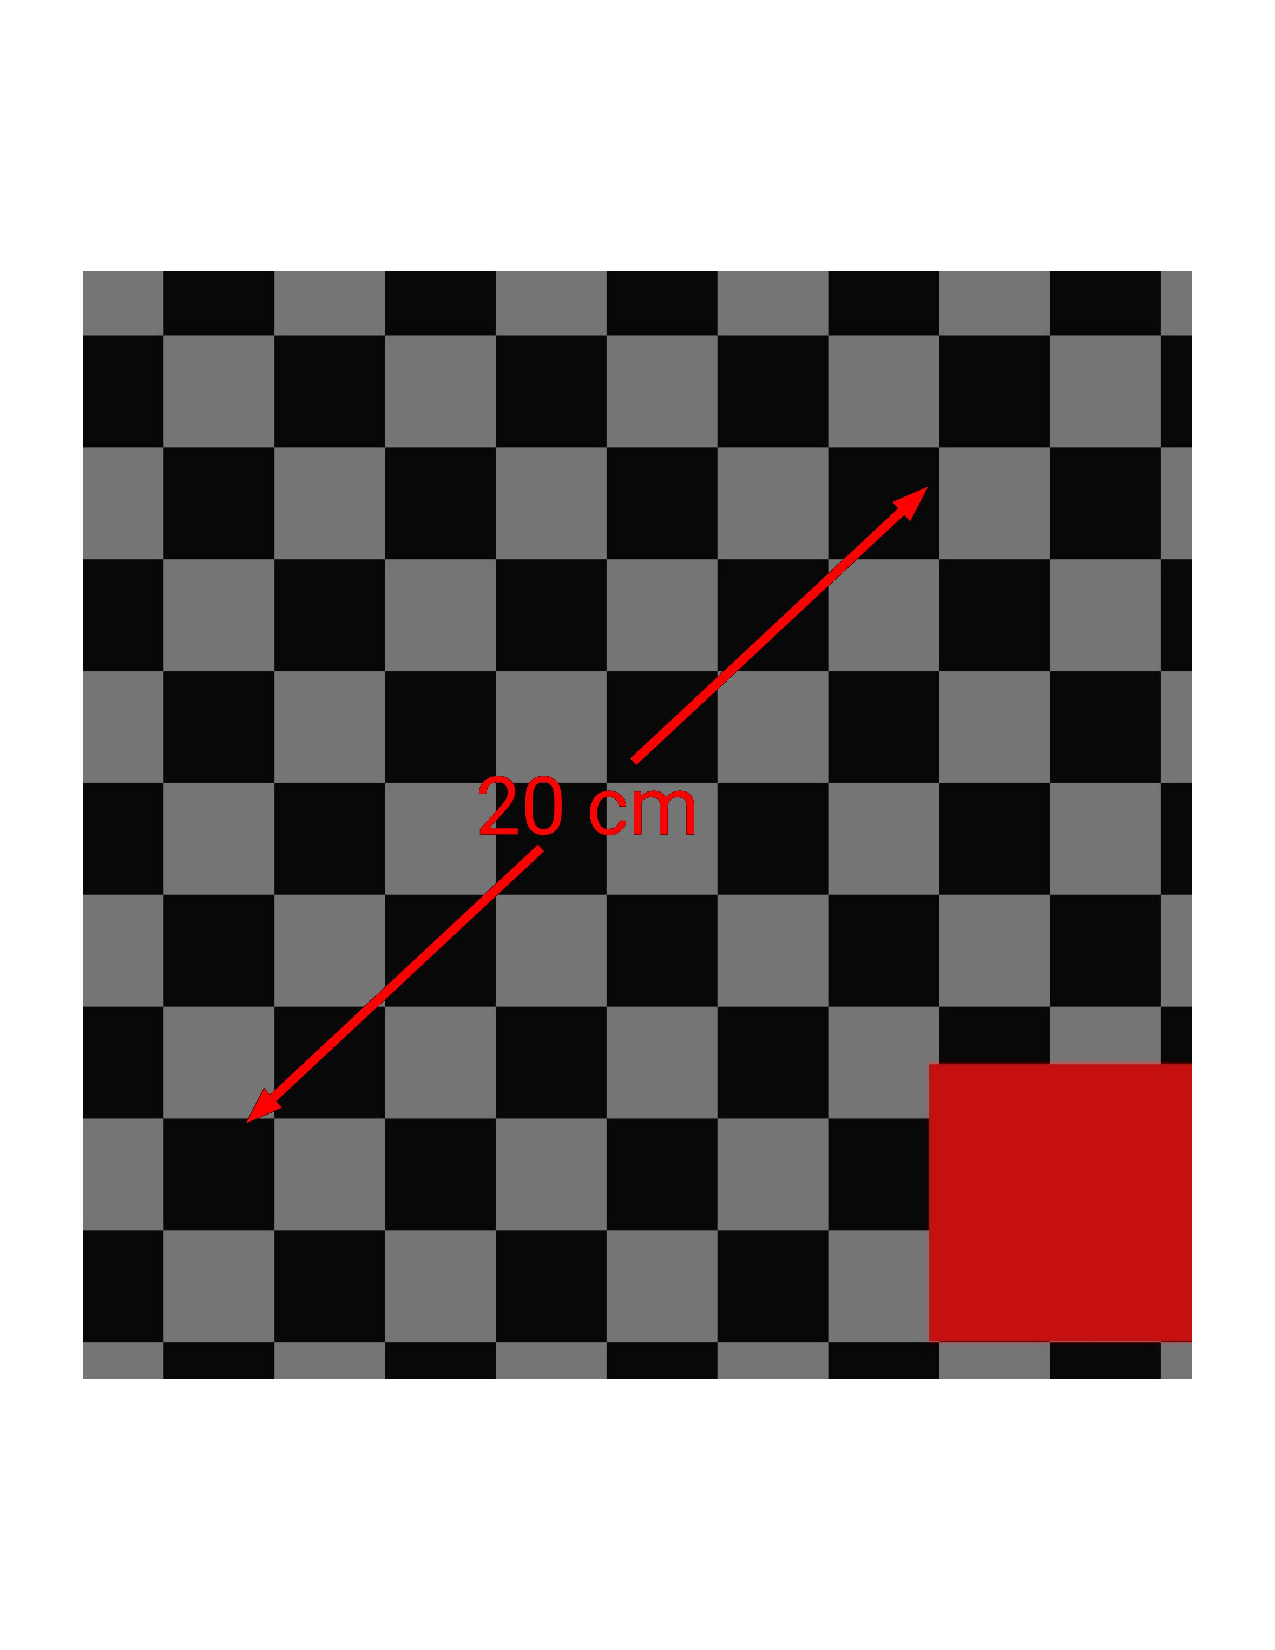
\includegraphics[keepaspectratio, width=\textwidth]{bosch/export}
  \caption{Exportierte PDF}
  \label{fig:bexport}
\end{figure}

\subsubsection{Evaluation}

Die App zeigt in einer Art Statusleiste am unteren Rand des Bildschirms den aktuellen Modus an, und gibt über einen auffordernden Text am oberen Bildschirmrand dem Nutzer eine Hilfestellung, was er im gerade ausgewählten Modus machen kann. \todo{screens} Hiermit deckt die App Nielsen \ref{itm:1} und \ref{itm:10} ausreichend ab. \\

Des Weiteren benutzt auch diese App universell verständliche Icons, um die wichtigsten Aktionen wiedererkennbar zu machen. So hat beispielsweise das Mülleimer-Icon in jedem Modus die Löschfunktion. \\

Im Gegensatz zu \textsc{Photo Measures} bietet diese App dem Benutzer die Möglichkeit seine Aktionen rückgängig zu machen, oder sie zu wiederholen. Dies ist ein deutlicher Vorteil seitens der Usability, da Fehler nicht so hart bestraft werden, als wenn keine Undo/Redo-Button vorhanden wären. \\

Fehler werden hier durch das Deaktivieren von Buttons, die im aktuellen Systemzustand nicht benutzbar sind, präventiv verhindert. Das Löschen von Formen ist beispielsweise nur dann möglich, wenn zuvor eine Form ausgewählt wurde.

Negativ fällt auch in dieser Alternative die fehlerhafte Gesten-Unterstützung auf. So sorgen Zoom-Gesten per Doppel-Tap zum unabsichtlichen Zeichnen einer Form, welche im Nachhinein wieder gelöscht werden muss. Außerdem verletzt die App Nielsen~\ref{itm:15}, da Änderungen in der Bildschirmausrichtung dafür sorgen, dass das Bild nicht wie erwartet seine Ursprungsausrichtung beibehält, sonder auch rotiert wird. 

\subsection{Image Meter - Messen im Foto}

\subsubsection{Vorstellung}
Die App \im{} von \emph{Dirk Farin} hat zur Zeit des Downloads (20. Januar 2018) bei insgesamt 2.764 abgegeben Bewertungen eine durchschnittliche Bewertung von 3,9 von 5 Sternen im Google Play-Store \citep{FarinIM}.
Hierbei haben 72\% (1324 + 654) der Bewertungen vier oder fünf, und nur 28\% (289 + 154 + 343) 3 oder weniger Sterne. \\
Dies ist im Vergleich zu den aderen Apps, die im Play-Store unter dem Suchbegriff ``Aufmaße'' frei erhältlich sind, eine vergleichweise hohe Bewertung, und macht diese App zu einer der beliebtesten in der Kategorie \emph{Aufmaße}.
Selbst beschreibt der Entwickler die App im Play-Store wie folgt \citep{FarinIM}:

\begin{quote}
  ``ImageMeter erlaubt das Beschriften Ihrer Fotos mit Längen-, Winkel- und Flächenmaßen sowie Text.
  Das ist viel einfacher und anschaulicher als aufwändig eine Skizze zu zeichnen.''
\end{quote}

\noindent
Beim Start der App wird dem Benutzer der sogenannte ``Tipp des Tages'' angezeigt. \\

\begin{wrapfigure}{R}{0.5\textwidth}
  \centering
  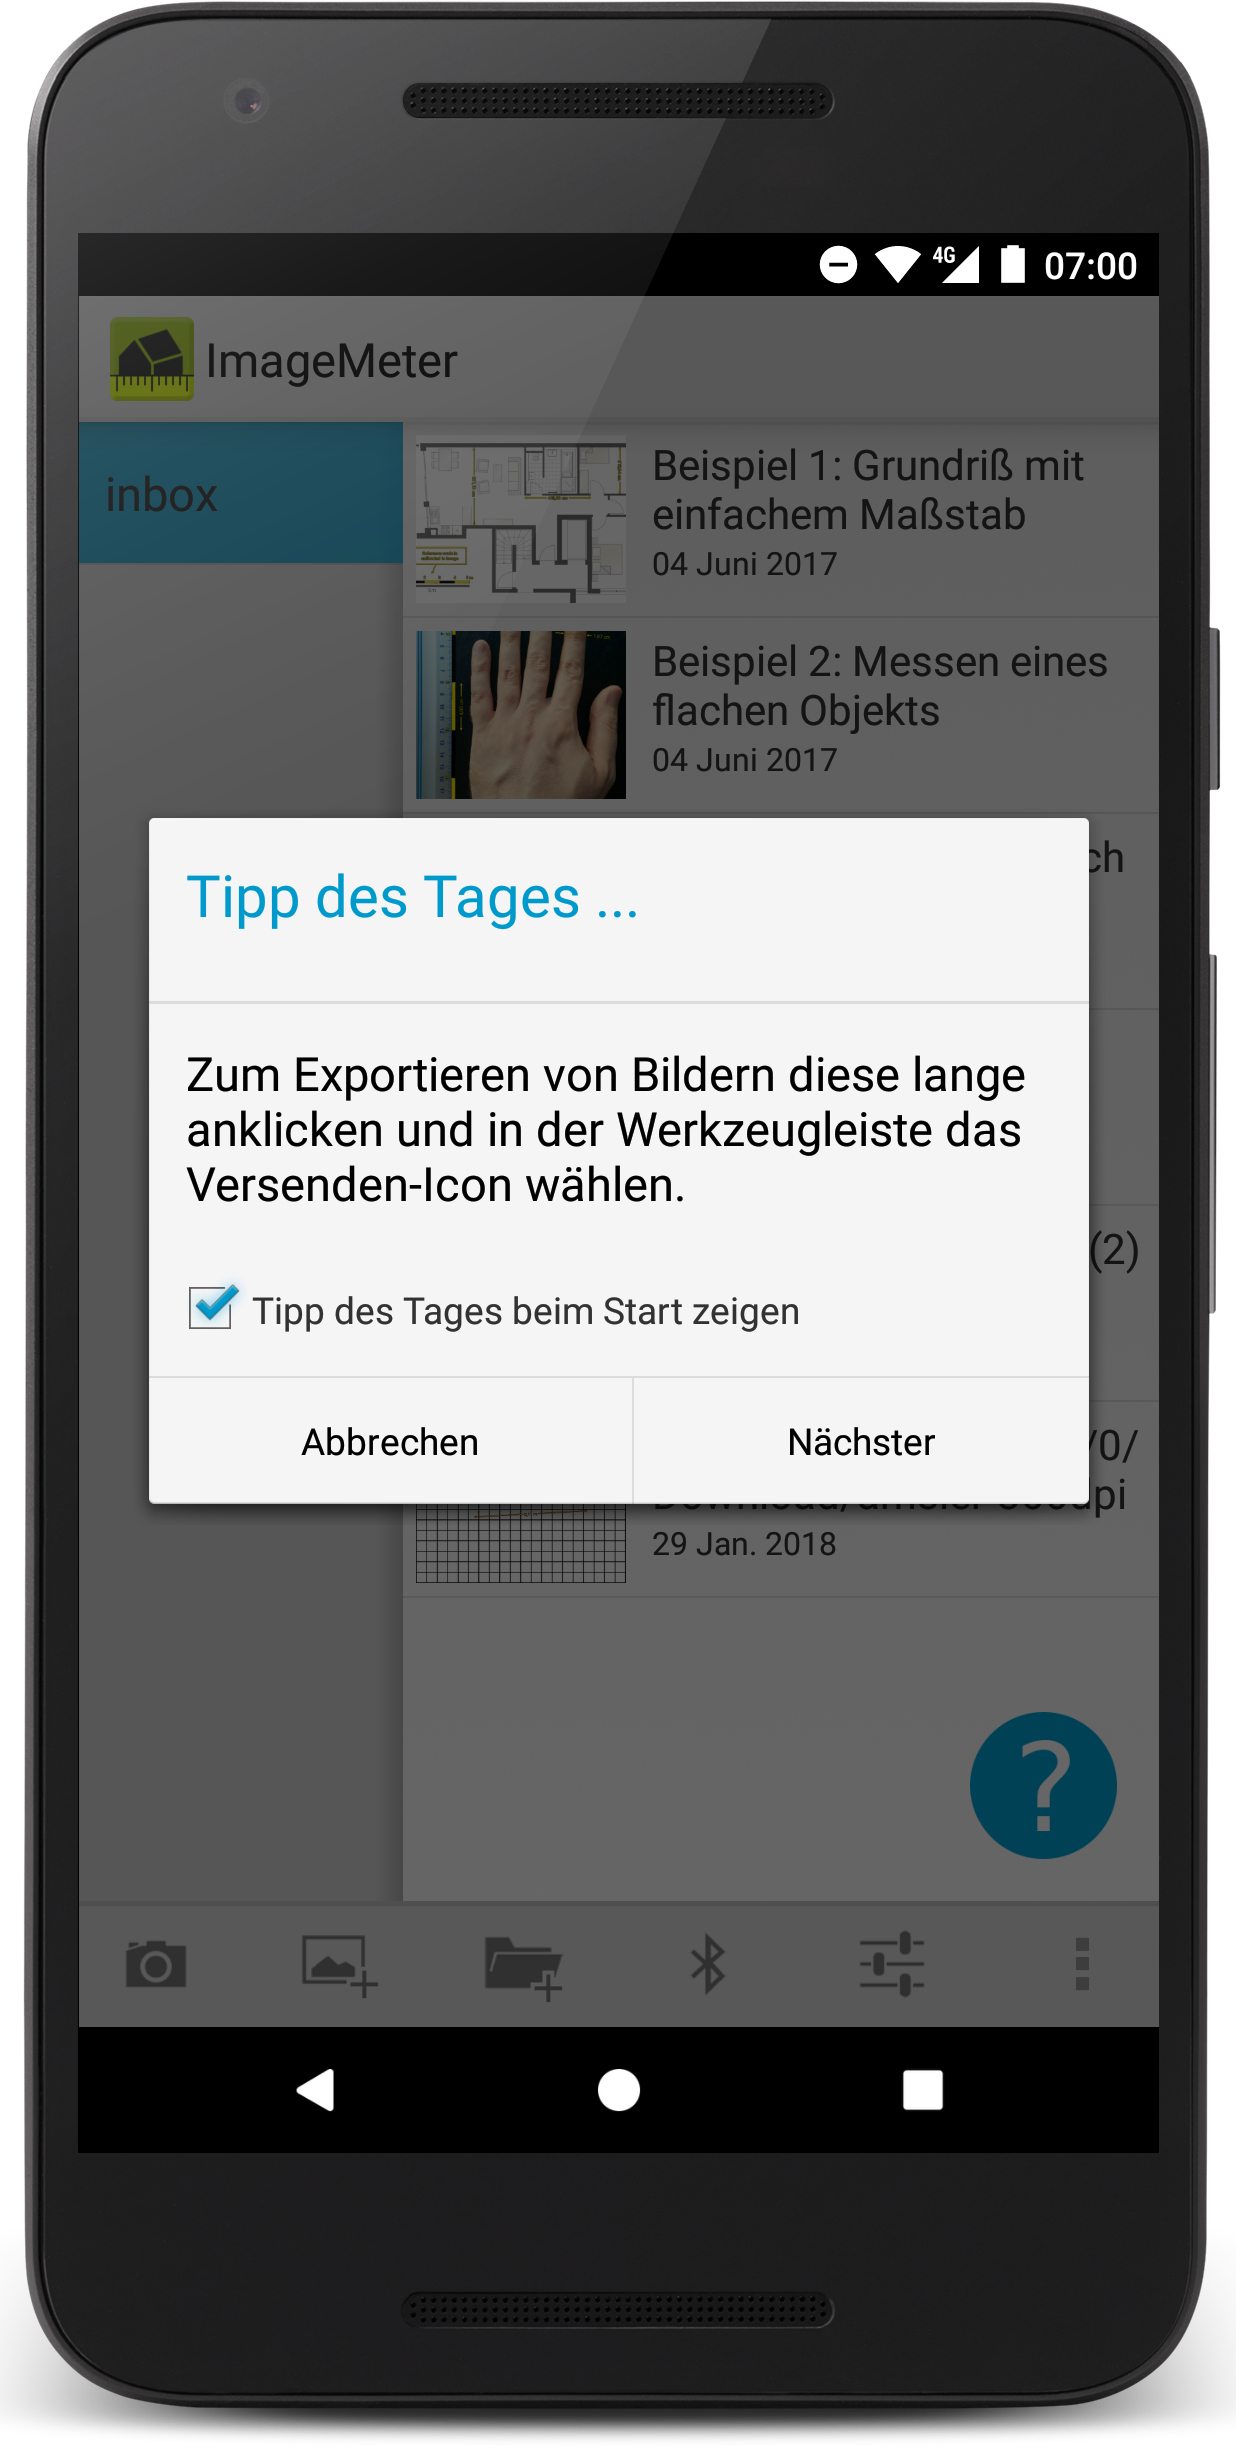
\includegraphics[keepaspectratio, width=0.5\textwidth]{image_meter/tip}
  \caption{``Tipp des Tages'' beim Start der App}
  \label{fig:imtip}
\end{wrapfigure}

Dieser enthält Informationen zu bestimmten Funktionen der App, wie zum Beispiel dem Exportieren von Bildern (siehe \autoref{fig:imtip}).
Hier hat der Nutzer die Möglichkeit sich weitere Tipps anzusehen, oder diese durch das Entfernen des Hakens in der Checkbox ``Tipp des Tages beim Start zeigen'' dauerhaft zu deaktivieren. \\

Sobald der Dialog zum ``Tipp des Tages'' geschlossen wurde, bietet sich über die Aktionsleiste am unteren Bildschirmrand die Möglichkeit, ein neues Bild aufzunehmen, oder direkt eines aus der Galerie zu importieren (siehe \autoref{fig:immenu}).
Das ausgewählte Bild wird nach erfolgreichem Import in die App im Hauptmenü an die Bilderliste angehangen. \\

Hier gelangt der Benutzer durch einen Klick auf das gewünschte Bild in eine neue Bildschirmöberfläche, in der Aufmaße eingezeichnet werden können (siehe \autoref{fig:imdraw})
In dieser Umgebung wird zusätzlich zum Bild noch eine Statusleiste am unteren Bildschirmrand und ein darüber befindlicher ``Floating Action Button'' \todo{ref} mit einem Fragezeichen-Symbol angezeigt.
Beim Klick auf diesen schwebenden Button öffnet sich eine Hilfe-Seite, in der zu den verschiedenen Funktionalitäten der App häufig gestellte Fragen, und deren Antworten zu lesen sind. \\

Zusätzlich zu dieser Hilfestellung, wird dem Benutzer beim Auswählen des ``Zeichen-Modus'' ein erklärender Text über der Statusleiste angezeigt (siehe \autoref{fig:imdraw}), der genau beschreibt, welche Aktion der Nutzer in diesem Systemzustand durchführen kann bzw. soll. \\

\begin{figure}[h]
  \centering
  \begin{subfigure}[t]{0.4\textwidth}
    \includegraphics[keepaspectratio, width=\textwidth]{image_meter/menu}
    \caption{Hauptansicht der App}
    \label{fig:immenu}	
  \end{subfigure}
  \begin{subfigure}[t]{0.4\textwidth}
    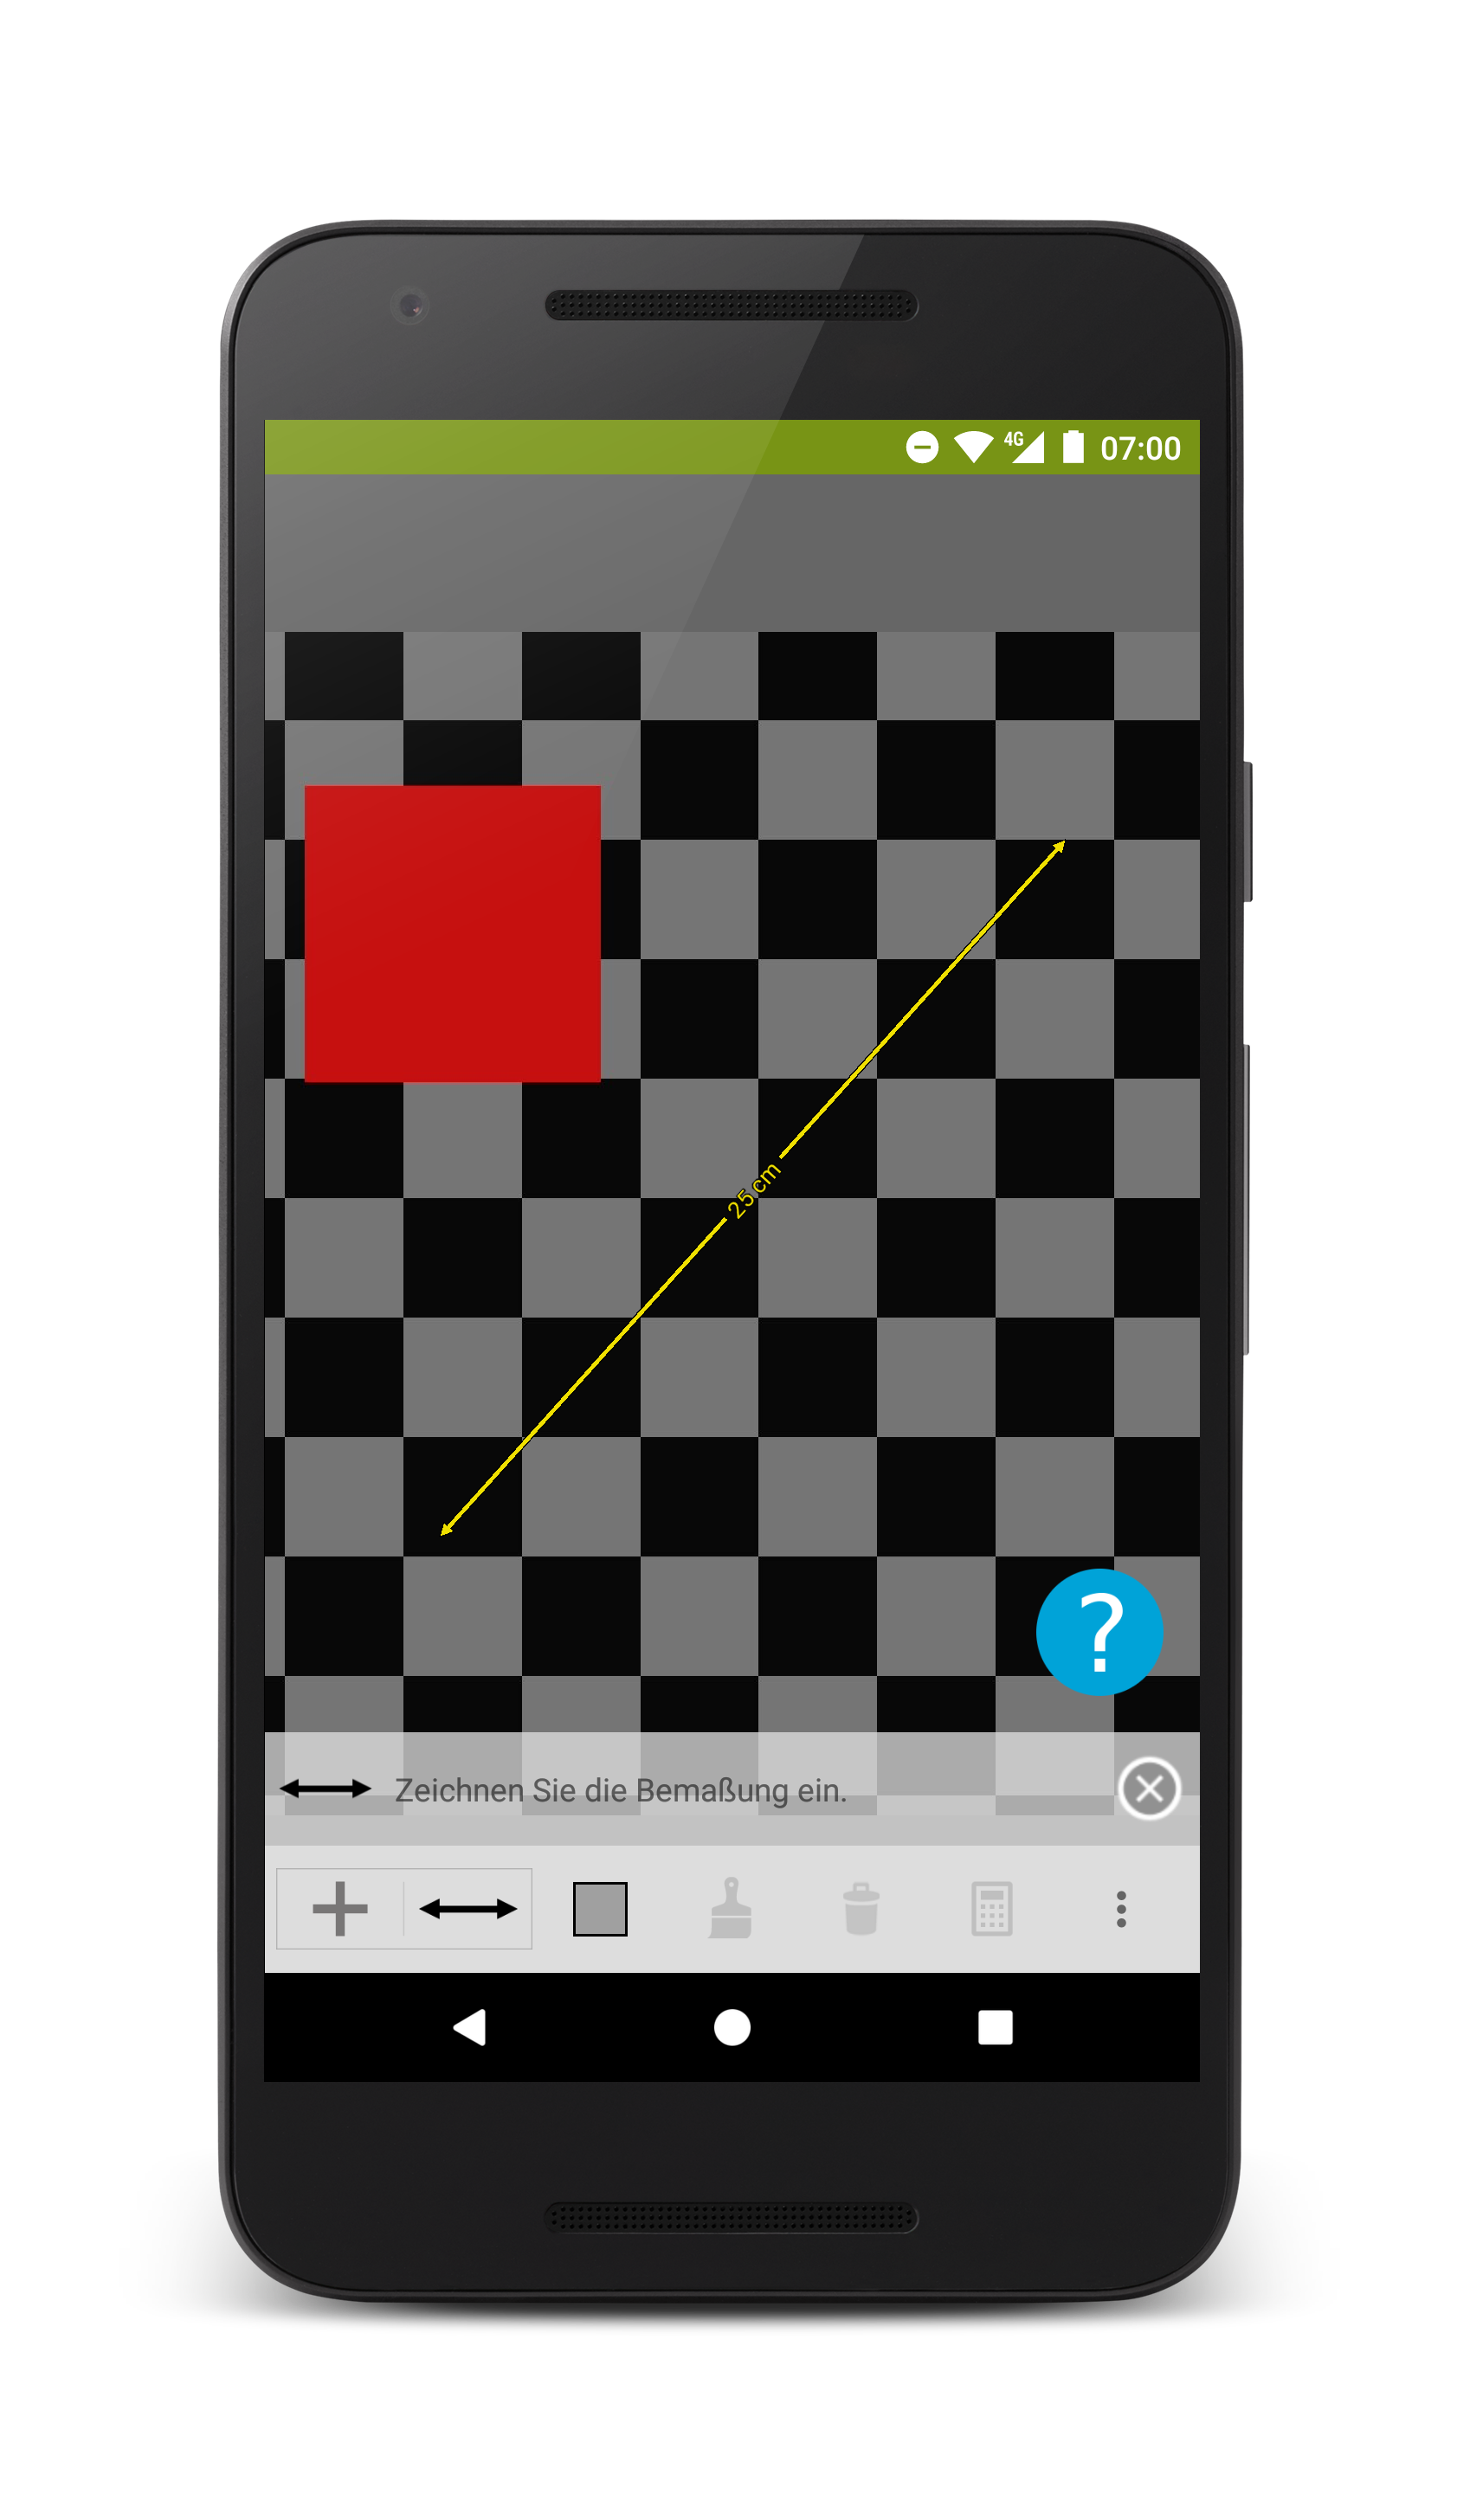
\includegraphics[keepaspectratio, width=\textwidth]{image_meter/draw}
    \caption{Aufmaße-Funktion mit eingezeichneter Form} 
    \label{fig:imdraw}	
  \end{subfigure}
  \caption{\im{} nach dem Start der App und in der Aufmaß-Funktion}
\end{figure}

\noindent
Zudem kann der Nutzer über die Statusleiste die gewünschte Form und deren Farbe auswählen.
Bereits eingezeichnete Formen können im Nachhinein wieder vergrößert bzw. verkleinert und in ihrem Aussehen verändert werden. \\

Des Weiteren werden nur die Funktionen, die zum jeweiligen Systemzustand ausführbar sind (z.B. Löschen und Textändernungen nur wenn Form ausgewählt), in der Statusleiste angezeigt.
Die App bietet die Möglichkeit aus sieben Formen - zehn in der Pro-Version - auszuwählen, und diese in das Bild einzuzeichnen.
Zusätzlich kann man in dieser App Gebrauch von Referenzpunkten machen, die es der App ermöglichen, neu eingezeichnete Formen automatisch mit Messwerten zu versehen.
Versehentlich ausgeführte Aktionen können durch einen Undo- bzw. Redo-Button in der Statusleiste rückgängig gemacht bzw. wiederholt werden. \\

Auch in dieser App lassen sich gespeicherte Bilder zu einem späteren Zeitpunkt weiter bearbeiten.
Außerdem können mehrere Bilder gleichzeitig zusammen in einer \emph{PDF} exportiert werden.

\subsubsection{Evaluation}

Hilfe und Dokumentation (Nielsen~\autoref{itm:N10}) werden in dieser App in Form des ``Tipp des Tages'' Dialogs (siehe \autoref{fig:imtip}), welcher sich zum Start der App zeigt, und durch eine dedizierte Benutzeroberfläche, die man über den Floating Action Button erreicht, bereit gestellt.

\begin{wrapfigure}{R}{0.5\textwidth}
  \centering
  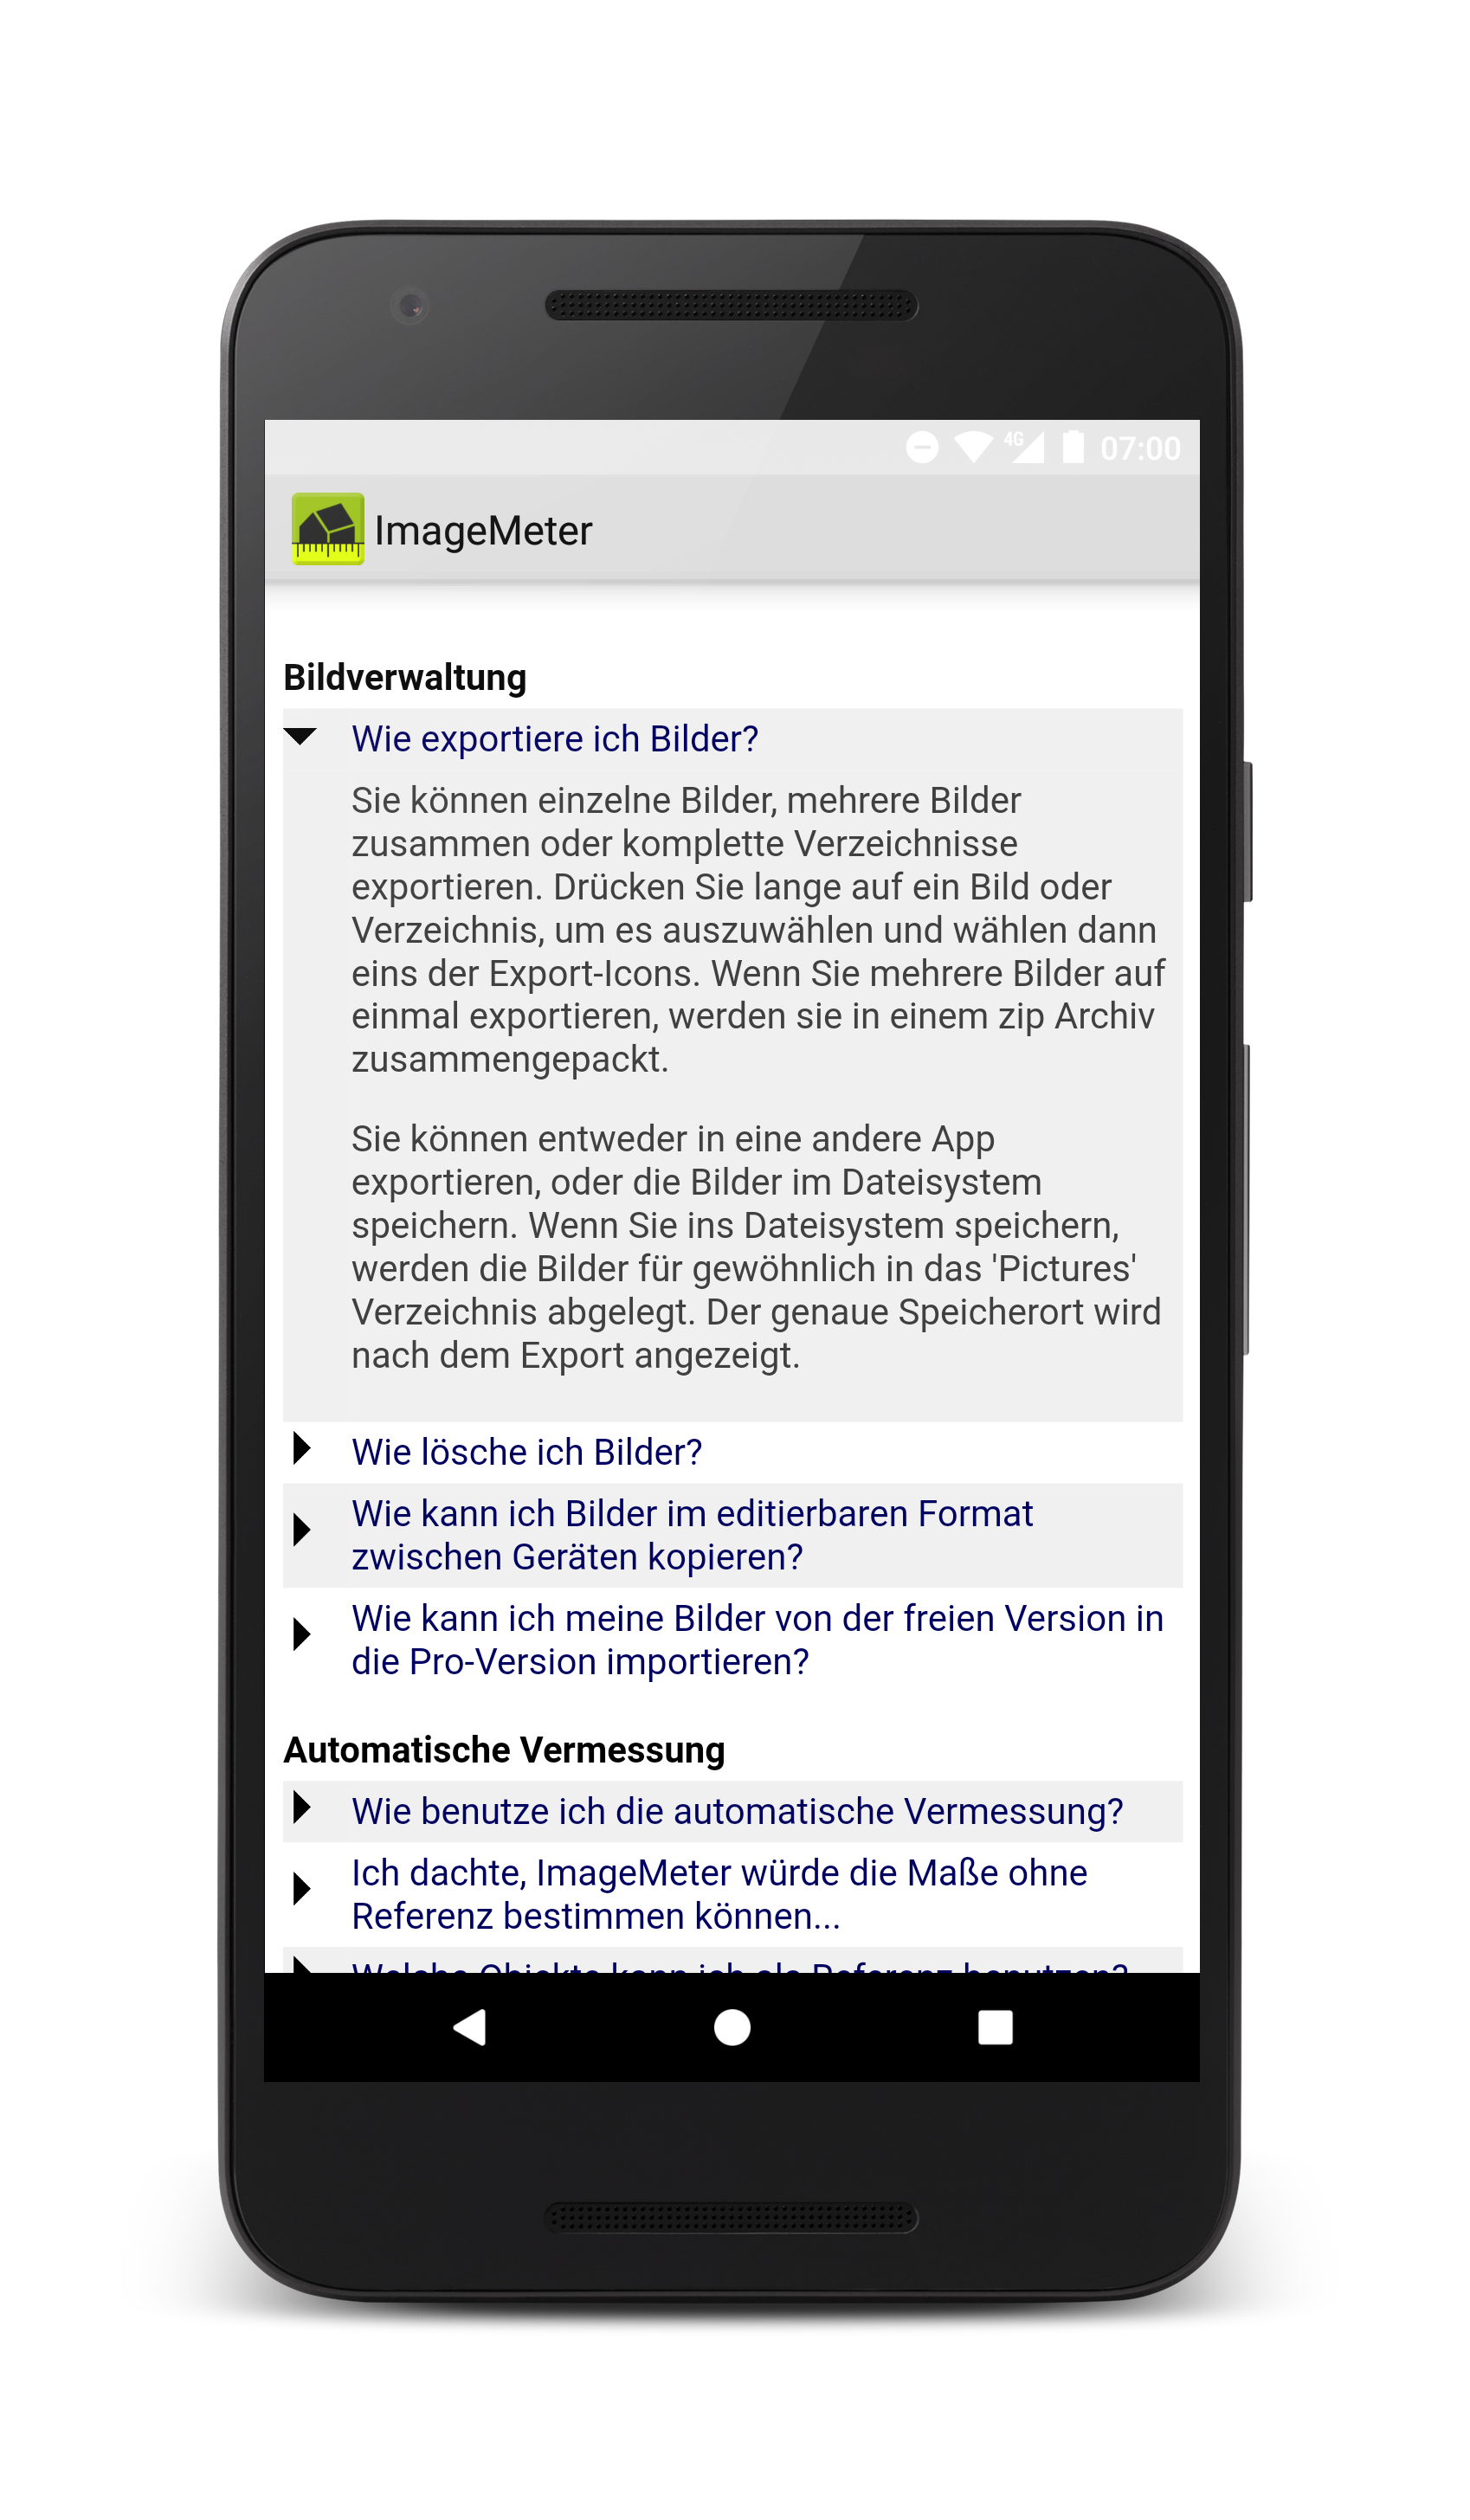
\includegraphics[keepaspectratio, width=0.5\textwidth]{image_meter/faq}
  \caption{Hilfeoberfläche der App}
  \label{fig:imfaq}
\end{wrapfigure}

Hierbei bietet die Hilfeoberfläche Antworten auf eine vorgegebene Menge Fragen zu den verschiedenen Funktionen der App (siehe \autoref{fig:imfaq}). \\

Die Statusleite zeigt zu jedem Zeitpunkt den ausgewählten Modus und die verfügbaren Aktionen an, und gibt dem Benutzer so eine angemessene und verständliche Rückmeldung über den aktuellen Systemzustand der App (Nielsen~\autoref{itm:N1} \& \autoref{itm:N5}). \\

Formen können, nachdem sie in das Bild gezeichnet wurden, zu einem späteren Zeitpunkt in ihrem Aussehn und ihrer Größe verändert werden. Zusätzlich dazu gibt es in den Einstellungen der App weitere Punkte, um diese den eigenen Benutzungsbedürfnissen anzupassen.
So kann zum Beispiel eingestellt werden, ob Maßeinheiten angezeigt werden sollen, welche metrischen Einheiten benutzt werden sollen, oder wie viele Dezimalstellen für Messwerte verwendet werden solle.
Dies erlaubt nicht nur eine flexible Benutzung der App, sondern sorgt gleichzeitig für eine potentielle Effizienzsteigerung, da die App nur einmal zu Beginn der Benutzung den Vorstellungen entsprechend konfiguriert werden muss (Nielsten~\autoref{itm:N7}) \\

Die App versucht Situationen, in denen Fehler auftreten könnten, präventiv zu vermeiden.
Hierzu werden Aktionen, die beim Ausführen im aktuellen Systemzustand zu einem Fehler führen würden, ausgegraut und sind nicht auswählbar (Nielsen~\autoref{itm:N5} \& \autoref{itm:N9}).

\begin{wrapfigure}{R}{0.5\textwidth}
  \centering
  \includegraphics[keepaspectratio, width=0.5\textwidth]{image_meter/bar}
  \caption{Statusleiste in der Aufmaßfunktion}
  \label{fig:imbar}
\end{wrapfigure}

Das Ausgrauen der unbenutzbaren Aktionen führt jedoch in Kombination mit den anderen verwendeten Farben in der Statusbar schnell zu Verwirrung.
So werden hier zwei verschiedene Grautöne benutzt, die sich nur minimal unterscheiden (siehe \autoref{fig:imbar}). \todo{bisschen mehr hierzu} \\

Über einen Undo- bzw. Redo-Menüpunkt hat der Benutzer die Möglichkeit, ungewollte oder fehlerhafte Eingaben zu revidieren, oder Aktionen zu wiederholen (Nielsen \autoref{itm:N3}).
Bei der Benutzung im Hochformat sind diese Menüpunkte jedoch nicht offensichtlich erkennbar, da sie in dem Overflow-Menü \todo{def} an der rechten Seite der Statusbar versteckt sind (siehe \autoref{fig:imbar}).
Der Benutzer muss hier also durch Zufall schon einmal das Overflow-Menü ausgeklappt haben, um zu wissen, dass sich dort die Optionen zum Undo bzw. Redo befinden. \\

Ein positiver Aspekt dagegen liegt beim adäquaten Umgang mit Unterbrechungen, sowie der Unterstützung verschiedener Bildschirmausrichtungen (Nielsen~\autoref{itm:N11} \& \autoref{itm:N15}).
Beim Pausieren und Drehen der App gehen keine Informationen, wie bereits eingezeichnete Formen oder eingetragene Messwerte verloren, und das Bild bleibt stets in der erwarteten Ausrichtung. 

\begin{wrapfigure}{R}{0.5\textwidth}
  \centering
  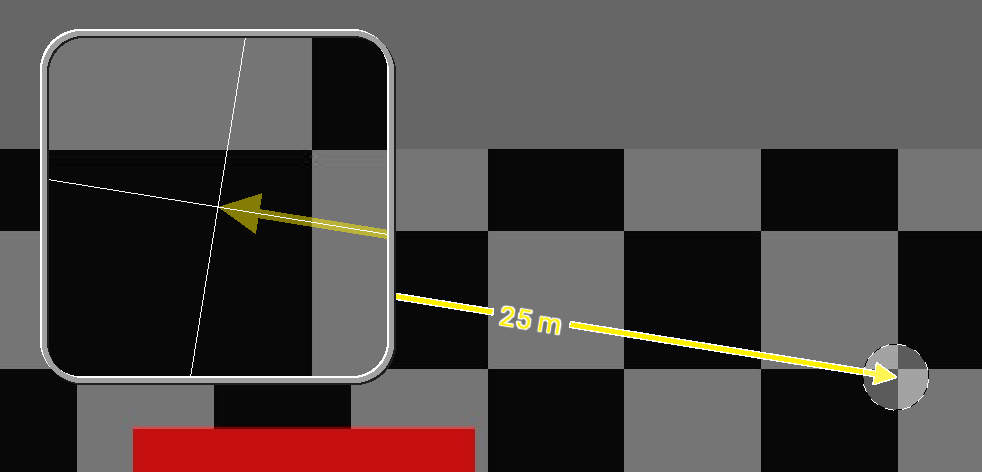
\includegraphics[keepaspectratio, width=0.5\textwidth]{image_meter/lensebug}
  \caption{Zoom-Linse verdeckt Zeichenbereich}
  \label{fig:imlense}
\end{wrapfigure}

Hinzukommend wird der zusätzliche Bildschirmplatz der sich im Querformat ergibt genutzt, um alle Elemente der Statusleiste anzuzeigen, ohne Aktionen im Overflow-Menü zu verstecken. \\

Eine positive Benutzererfahrung ergibt sich aus der einfachen und effizienten einhändigen Handhabung in Kombination mit einer fehlerfreien Gesten-Unterstützung zur Navigation im Bild. (Nielsen~\autoref{itm:N13}, \autoref{itm:N16} \& \autoref{itm:N17}). \\

Außerdem bedient sich auch diese App beim Zeichnen von Formen einer Zoom-Linse, welche den Bereich um die Fingerposition vergößert darstellt.
Negativ fällt bei der Umsetzung dieser Funktion jedoch auf, dass die Zoom-Linse statisch in der oberen linken Ecke angezeigt wird, und sich bei Kollision mit dem Zeichenfinger nicht bewegt.
Dies kann dazu führen, dass der gezoomte Bereich beim Zeichnen die Form verdeckt und seine eigentlichen Aufgabe als Hilfestellung zur genaueren und schnelleren Zeichnung verfehlt (siehe \autoref{fig:imlense}). \\

Die App ermöglicht das Teilen von vorhandenen Bildern in diese, bietet beim Exportieren jedoch keine Möglichkeit die eingetragenen Messwerte als Meta-Daten beizubehalten.
So wäre es zwar möglich, Bilder aus der bestehenden Android-App an \im{} zu teilen, diese zu bearbeiten und anschließend abzuspeichern. 
Aber es gäbe keine Möglichkeit aus der bestehenden Android-App auf die eingetragenen Messwerte zuzugreifen, und diese für einen nachgeschalteten Diesnt aufzubereiten. \\

Zusammenfassend kann gesagt werden, dass die App \im{} von \emph{Dirk Farin} die Nielsen-Heuristiken überwiegend positive erfüllt.
Die versteckten Undo/Redo-Funktionalität und die Verwirrung des Nutzers durch die Verwendung ähnlicher Grautöne für unterschiedliche Aktionen in der Statsubar sind bei der Evaluation als Negativaspekte identifiziert worden.
Besonders diese beiden Punkte in Kombination mit der fehldenden Einführung bzw. Hilfe-Stellung beim ersten Start der Aufmaß-Funktion, wirken sich negativ auf die initiale Benutzererfahrung der App aus.
So muss der Benutzer, falls sich Fragen während des Einzeichnens von Formen ergeben, die aktuelle Oberfläche verlassen, in eine andere Oberfläche wechseln, und dort die passende Frage suchen. 

Hierdurch können Fehler entstehen, die mit der Nutzung einer Android-App für die Aufmaßerfassung verhindert werden sollten.

\subsection{Photo Measures}
hallo


\section{Auswertung der Evaluationsergebnisse}
\begin{sidewaystable}[ht]
  \centering
  \caption{Vergleich der Lösungsalternativen}
  \vspace*{10px}
  \label{tab:nielsen}
  \begin{tabular}{|r|l|c|c|c|}
    \hline
    &								          &       \mm{}   &   \emph{ImageMeter}	  &       \pm{}     \\
    \toprule
    \multirow{10}{*}{\rot{\textbf{Nach \cite{Nielsen94}}}}
    & \hyperref[itm:N1]{1. Sichtbarkeit des Systemzustandes}				&       \po 		&    \po 			&       \po       \\ \cline{2-5} 
    & \hyperref[itm:N2]{2. Übereinstimmung zwischen System und realer Welt} 				&       \po  		&    \po  		&       \po		    \\ \cline{2-5}
    & \hyperref[itm:N3]{3. Benutzerkontrolle- und freiheit} 				&       \po 		&    \xmark	  &       \xmark    \\ \cline{2-5} 
    & \hyperref[itm:N4]{4. Konsistenz und Standards} 				&       \po  		&    \po			&       \po    \\ \cline{2-5}
    & \hyperref[itm:N5]{5. Fehlervorbeugung} 				&       \po  		&    \po			&       \po       \\ \cline{2-5} 
    & \hyperref[itm:N6]{6. Wiedererkennung statt Erinnern} 				&       \po 		&    \xmark		&       \po    \\ \cline{2-5} 
    & \hyperref[itm:N7]{7. Flexibilität und Effizienz der Benutzung} 				&       \xmark  &    \po			&       \po       \\ \cline{2-5} 
    & \hyperref[itm:N8]{8. Ästethisches und minimalistisches Design} \cc    &       \ccnl   &    \ccnl    &       \ccnl     \\ \cline{2-5}
    & \hyperref[itm:N9]{9. Erkennbarkeit, Diagnose und Erholung von Fehlern} 				&       \po   	&    \po 			&       \xmark    \\ \cline{2-5} 
    & \hyperref[itm:N10]{10. Hilfe und Dokumentation} 			&       \po  		&    \xmark		&       \po       \\
    \midrule
    \multirow{8}{*}{\rot{\textbf{Erweitert nach \cite{Machadoeto13, Bertini09}}}}
    & \hyperref[itm:N11]{11. Adäquater Umgang mit Unterbrechungen} 			&       \po   	&    \po 			&       \po       \\ \cline{2-5} 
    & \hyperref[itm:N12]{12. Fokussieren von Informationen} 			&       \po   	&    \po 			&       \po    \\ \cline{2-5} 
    & \hyperref[itm:N13]{13. ``Joy of Use''}			 	&       \xmark  &    \po  		&       \xmark       \\ \cline{2-5} 
    & \hyperref[itm:N14]{14. ``Don't lie to the user''} \cc   &       \ccnl   &    \ccnl    &       \ccnl     \\ \cline{2-5}
    & \hyperref[itm:N15]{15. Unterstützung verschiedener Bildschirmausrichtungen} 			&       \xmark  &    \po		  &       \po     	\\ \cline{2-5}   
    & \hyperref[itm:N16]{16. Ergonomische Gestaltung der physischen Interaktion} 			&       \xmark  &    \po  		&       \xmark    \\ \cline{2-5} 
    & \hyperref[itm:N17]{17. Einfache Eingabe, Lesbarkeit und Übersichtlichkeit} 			&       \po  		&    \po  		&       \po   		\\ \cline{2-5} 
    & \hyperref[itm:N18]{18. Stelle Privatheit sicher} \cc   &       \ccnl   &    \ccnl    &       \ccnl     \\
    \midrule
    \multirow{6}{*}{\rot{\textbf{Unternehmensanforderungen}}}
    &&&& \\
    & \hyperref[itm:integration]{Integration der App in eine vorhandene Systemarchitektur}  &      	\xmark	&    \xmark   &       \xmark    \\
    &&&& \\ \cline{2-5}
    &&&& \\ 
    & \hyperref[itm:export]{Export des annotierten Bildes und der Meta-Daten}    &      	\xmark	&    \xmark		&       \xmark  \\
    &&&& \\ \bottomrule
  \end{tabular} \\
  \vspace*{10px}
  Bei der Bewertung nicht berücksichtigte Kriterien sind in \textcolor{gray}{grau} hinterlegt und mit \nl{} gekennzeichnet. \\
  Gut umgesetzte Kriterien sind mit \po{} und schlecht umgsetzte Kriterien mit \xmark{} markiert.
\end{sidewaystable}


Wie sich in \autoref{sec:evaluation} gezeigt hat, hat jede der drei vorhandenen Lösungsalternativen verschiedene Vor-, aber auch Nachteile.
Besonders auffällig hierbei ist die fehlerhafte Umsetzung der \emph{Pinch-Geste} zum Zoomen des Bildes in den beiden Apps \mm{} und \pm{}.
Diese fehlerhafte Umsetzung der \emph{Pinch-Geste} führt dazu, dass der Nutzer Formen löschen muss, die unabsichtlich während des Zoomens gezeichnet wurden.
Insbesondere bei der App \pm{} führt dieser Fehler zu einem enorm schlechten Anwendererlebnis, da es keine Undo-Funktion gibt, um die fehlerhaft eingezeichnete Form schnell rückgängig zu machen.
Hier muss die Form zuerst markiert, und anschließend über einen Klick auf das Mülleimer-Icon in der Statusleiste gelöscht werden, bevor der Nutzer mit der eigentlichen Arbeit fortfahren kann. \\

Außerdem ist in \autoref{sec:evaluation} aufgefallen, dass alle drei Apps eine Zoom-Linse benutzen, um den Bereich, der von dem Finger beim Zeichnen einer Form bedeckt wird, vergrößert an einer anderen Stelle des Bildschirms darzustellen.
Hierdurch kann der Nutzer schnell und präzise Formen in das Bild zeichnen, ohne jedes Mal den Finger hochnehmen zu müssen, um zu sehen, bis wohin die Form schon gezeichnet wurde.
Die Umsetzung dieser Zoom-Linse ist in den beiden Apps \mm{} und \pm{} besser gelöst als in \im{}.
Hier ist die Position der Zoom-Linse statisch in der oberen linke Ecke des Bildschirms fixiert, und bewegt sich auch bei der Kollision mit der gezeichneten Form nicht. \\

Alle drei Apps benutzen Icons, um den Systemzustand und die darin ausführbaren Aktionen darzustellen.
Zusätzlich deaktivieren alle drei Apps die Aktionen, welche im aktuellen Systemzustand nicht ausführbar sind bzw. zu Fehlern führen würden.
Dieses Deaktivieren bestimmter Icons wird bei den beiden Alternativen \mm{} und \pm{} intuitiv verständlich umgesetzt, wohingegen die App \im{} durch die Verwendung ähnlicher Grautöne für deaktivierte und normale Icons für Verwirrung beim Benutzer sorgt. \\

Ein weiterer wichtiger Aspekt, der von keiner der evaluierten Apps erfüllt wurde, ist die Integration in eine bereits bestehende Systemarchitektur bzw. der Export der bearbeiteten Bilder ohne die eingetragenen Messwerte als Meta-Daten zu verlieren. 
Hierbei hat die App \im{} im Vergleich zu den anderen beiden Alternativen besser abgeschnitten, da diese das Teilen von Bilder aus einer bestehenden App in sich selber zulässt.
Die Integration bleibt jedoch bei allen drei Apps nur sehr mühsam möglich, da beim Export der bearbeiteten Bilder die Messwerte nicht mehr als Meta-Daten vorliegen.
Durch den Export werden nämlich sämtliche eingetragene Messwerte und Formen in das Bild geschrieben, und müssten anschließend wieder mühsam aus dem Bild extrahiert werden. \\

Alle Evaluationsergebnisse, die in diesem Kapitel gesammelt werden konnten, sollen im nächsten Kapitel auf die Konzeption einer eigenen Android-Applikation angewandt werden.
Hierbei sollen Aspekte, die während der Evaluation als besonders positiv aufgefallen sind, in die Konzeption der eigenen App einfließen, und bereits identifizierte Usability-Probleme vermieden werden.
\todo{ein bisschen ausbauen}
